% =====================================================================
% Paper 2, written in the same plain style as the author's ThesisProj draft.
%
% Every number here comes from a scored, pre-registered experiment. The
% pre-registrations and their scores are in reports/p16 through reports/p22.
%
% Claims are worded to match what the experiments support. In particular:
%   * the paper claims training-design SENSITIVITY, not a proven mechanism;
%   * the paired per-seed changes are the result; the endpoints are not
%     separated from zero on three seeds and the paper says so;
%   * the loss-imbalance mechanism is cited, not claimed;
%   * the log-domain loss is reported as "no resolved difference".
% =====================================================================
\documentclass[journal]{IEEEtran}
\IEEEoverridecommandlockouts

\usepackage{amsmath,amssymb,amsfonts}
\usepackage{graphicx}
\usepackage{booktabs}
\usepackage{url}

\DeclareMathOperator{\rank}{rank}
\newcommand{\bG}{\mathbf{G}}
\newcommand{\bS}{\mathbf{S}}
\newcommand{\bB}{\mathbf{B}}
\newcommand{\bW}{\mathbf{W}}
\newcommand{\bZ}{\mathbf{Z}}
\newcommand{\bg}{\mathbf{g}}
\newcommand{\CN}{\mathcal{CN}}
\newcommand{\Hank}{\mathcal{H}}

\begin{document}

\title{Training-Design Sensitivity of Structural-Prior\\
Gains in Unrolled Channel Estimation for\\
Rydberg Atomic Receivers}

\author{Abdullah~Haatim%
\thanks{A.~Haatim is with the Department of Electrical and Electronics
Engineering, Birla Institute of Technology and Science, Pilani~--- Pilani
Campus, India (e-mail: f20220519@pilani.bits-pilani.ac.in).}}

\maketitle

\begin{abstract}
A common way to improve an unrolled channel estimator is to add a structural
constraint inside the network, and the improvement that follows is usually
credited to that constraint. This paper shows that in magnitude-only channel
estimation for Rydberg atomic receivers, such a comparison does not by itself
establish the credit, because the measured improvement depends strongly on how
the two networks were trained. A training loss averaged over a wide
signal-to-noise ratio range is dominated by its low-noise-ratio tail; in our
setting $89.7\%$ of the measured gradient falls below $5$~dB, so any mechanism
that helps at high SNR can appear to supply information. We propose a
matched-adequacy control: measure how the gradient is shared across SNR,
retrain both the structured and the unstructured network with the imbalance
removed, and measure the difference again. Using three training designs with
three random seeds each, the structural gain above $5$~dB is $+1.286$~dB under
the conventional loss, close to zero when both networks are retrained on the
high-SNR range, and negative when the loss is corrected instead. Compared seed
by seed, the change from conventional training is $-1.27$ and $-1.46$~dB, and
both changes are clearly separated from zero, although the individual values
are not. We also show that a per-bin pattern survives where no single number
does, that correcting the loss is worth $+2.171$~dB over three seeds, and that
a simpler log-domain loss gives no resolved difference. All results are
simulation only.
\end{abstract}

\begin{IEEEkeywords}
Algorithm unrolling, channel estimation, evaluation methodology, phase
retrieval, Rydberg atomic receiver, structural priors.
\end{IEEEkeywords}

\section{Introduction}

\IEEEPARstart{U}{nrolling} an iterative estimator into a trained
network~\cite{gregor2010,monga2021} has become a standard method for channel
estimation, including for Rydberg atomic receivers, where the magnitude-only
readout makes the problem one of phase retrieval~\cite{xiao2026,cui2025}. A
common next step is to add an explicit structural constraint inside the
unrolled loop, such as a low-rank projection, and to report the resulting
improvement as evidence that the constraint supplies information the network
could not learn by itself.

This paper argues that such evidence is usually not decisive. The reason is a
convention that is so common it is rarely written down: the training loss is a
per-sample normalized error, averaged over a training set that spans a wide SNR
range.

The problem with this convention is easy to state. At low SNR the normalized
error of any estimator is large, and at high SNR it is small. When we average
them together, the large numbers dominate. The network therefore spends most of
its training effort on the low-SNR samples. The high-SNR samples receive very
little attention, so the network is not trained as well there as it could be.

Now suppose we add a structural constraint to this network. The constraint
helps most where the network was least trained, which is at high SNR. The
measured improvement is therefore large. But that improvement is at least
partly repairing a training problem, not supplying new information. An
experiment that does not control for this cannot tell the two apart.

\textbf{The imbalance itself is known, and we do not claim it.} Wiesmayr
\emph{et al.}~\cite{wiesmayr2023bler} state it directly for machine-learning
assisted detection and decoding: a system learns one set of parameters while
operating over a range of SNRs, the training data is drawn from that range, and
the total loss is then dominated by the low-SNR samples, because a small
relative improvement at low SNR changes the cost more than a large relative
improvement at high SNR. They propose SNR deweighting as the remedy. Work on
deep OFDM channel estimation has separately studied training on
SNR-restricted samples and reports the expected trade between low-noise and
high-noise accuracy~\cite{jameel2024ofdm}.

What we take from that work is the mechanism and the remedy. What is not taken
from it, and what this paper is about, is the consequence for
\emph{attribution}: a known training problem can create apparent evidence for a
structural constraint, so an uncontrolled comparison does not establish that
the constraint supplied the improvement. Wiesmayr \emph{et al.} identify the
problem and fix it; they do not ask what it does to the evidence.

The estimator studied here is our own. We built a Hankel-structured unrolled
network, measured an advantage at high SNR, and believed it. The control
described in Section~\ref{sec:protocol} was run to describe that advantage
better. It removed it instead, and we report that on our own method for the
same reason we would report it on anyone else's.

\section{System Model and Estimator}

\subsection{The Measurement}

We consider an uplink system with $K$ single-antenna users and one Rydberg
atomic receiver with $N$ vapour-cell receive elements in a uniform linear
array. The users transmit $P$ known pilot symbols, collected in
$\bS\in\mathbb{C}^{K\times P}$. A known reference field
$\bB\in\mathbb{C}^{N\times P}$ is applied at the receiver. The receiver
measures only the magnitude of the total field,
\begin{equation}
\bZ=\left|\bG\bS+\bB+\bW\right|,\qquad \bW_{np}\sim\CN(0,\sigma^2),
\label{eq:obs}
\end{equation}
where $|\cdot|$ is applied to every element and $\bG\in\mathbb{C}^{N\times K}$
is the unknown channel. The phase of the received field is not observed.

Each user's channel is a sum of $L_k$ plane waves across the array,
\begin{equation}
g_k[n]=\sum_{\ell=1}^{L_k}\alpha_{\ell,k}e^{-j(n-1)\psi_{\ell,k}},\qquad
\psi_{\ell,k}=\pi\sin\theta_{\ell,k},
\label{eq:chan}
\end{equation}
with $L_k$ selected between 3 and 7, following~\cite{xu2025}. The path gains
are scaled so that the total received power does not change with the number of
paths.

This paper studies the magnitude-only Rydberg architecture. A superheterodyne
Rydberg receiver recovers both amplitude and phase, and nothing here applies to
it.

\subsection{The Unrolled Estimator}

The classical baseline is the expectation--maximization Gerchberg--Saxton
iteration (EM-GS) of Cui \emph{et al.}~\cite[Alg.~2]{cui2025}, which adapts the
classical Gerchberg--Saxton scheme~\cite{gerchberg1972} to this receiver. The
unrolled estimator, which we call the URformer after~\cite{xiao2026}, replaces
$T=10$ iterations of EM-GS with $10$ learned layers. Each layer performs a
data-consistency step, then a learned filter, then a Transformer block acting
across users. The architecture is not a contribution of this paper; we use it
as the object of study.

\subsection{The Structural Step Being Tested}
\label{sec:model}

The constraint we evaluate is a single denoising step applied to the channel
estimate inside every layer. It is important to define it exactly, because it
is the thing being measured.

Let $\Hank$ be the map that takes a vector $\bg\in\mathbb{C}^N$ and writes its
sliding windows as an $(N-p)\times(p+1)$ Hankel matrix, with
$p=\lceil N/2\rceil-1$. Let $\Hank^{\dagger}$ average the antidiagonals, which
converts such a matrix back into a vector. Let $\Pi_r$ keep only the $r$
largest singular values. The structured network replaces each column $\bg_k$ of
the estimate by
\begin{equation}
\bg_k\leftarrow\Hank^{\dagger}\Pi_r\Hank\,\bg_k,\qquad r=7.
\label{eq:cadzow}
\end{equation}

Four properties of this step matter, and each is easy to overstate.

\textbf{It is a denoising step, not a projection.} Reducing the rank generally
destroys the Hankel pattern, and averaging the antidiagonals to restore that
pattern generally raises the rank again. One pass therefore does not land on
the set of matrices that are both Hankel and low rank. Applying it twice also
changes the answer a second time, so it is not idempotent, which a projection
must be.

\textbf{It is applied every time.} There is no gate and no rank selection. Every
layer applies \eqref{eq:cadzow} on every trial. Nothing in this paper tests a
structural estimator that decides when to apply itself, which is a different
method.

\textbf{Its gradient is approximated.} In the forward direction the network
computes \eqref{eq:cadzow} exactly. In the backward direction it treats the
step as if it were the identity. This is done because the exact derivative of a
truncated SVD contains terms of the form
$1/(\sigma_i^2-\sigma_j^2)$, which become meaningless when two singular values
are close together, while removing the step from the graph entirely would cut
the gradient path to all earlier layers. This approximation is a design choice
and is part of what is being measured.

\textbf{The two networks are otherwise identical.} Both have $1{,}586{,}900$
parameters, the same number of layers, the same optimizer and schedule, the
same data order, the same initialization and the same random seed. The step in
\eqref{eq:cadzow} adds no trainable parameters. We write
\begin{equation}
\Delta_H=\mathrm{NMSE}_{\mathrm{no\ structure}}-\mathrm{NMSE}_{\mathrm{structure}},
\end{equation}
so a positive $\Delta_H$ means the structural step helps.

\section{The Training Problem and the Control}
\label{sec:protocol}

\subsection{Where the Gradient Goes}

The training loss is the per-sample normalized error
$\|\hat\bG-\bG\|_F^2/\|\bG\|_F^2$, averaged over a batch drawn from the whole
SNR range. As explained in the introduction, this average is dominated by the
low-SNR samples. We measured how strongly.

We define the gradient share of an SNR bin $b$ as
\begin{equation}
q_b=\frac{\|g_b\|}{\sum_c\|g_c\|},
\end{equation}
where $g_b$ is the gradient of the loss computed on the samples in bin $b$
alone. We measure it over $24$ batches per bin, at the selected checkpoint,
using all trainable parameters.

Two cautions about this quantity are worth stating before we use it. First,
$\sum_b\|g_b\|$ is not the same as $\|\sum_b g_b\|$, so $q_b$ is a normalized
share of gradient sizes and not a fraction of the total gradient. Second, an
equal share across bins is a reference we chose, not a property that an optimal
solution must have.

Measured on our estimator, $89.7\%$ of the gradient comes from trials below
$5$~dB, and the per-bin share spans a factor of $30.0$ across the range.

This raises a concern: the high-SNR region may be receiving too little of the
training effort, so any mechanism that improves high-SNR behaviour can look as
though it added information. \textbf{A skewed share does not prove this by
itself.} A small gradient can also mean a region that is already fitted well.
Section~\ref{sec:logloss} gives a case where a network that performs well still
shows the same skew. The share is a reason to check, not a verdict.

\subsection{The Control}

We propose the following control, which is cheap, and which we recommend be run
before a structural constraint is credited.

\begin{enumerate}
\item Measure the per-bin gradient share of the training loss.
\item Retrain \emph{both} the structured and the unstructured network with the
imbalance removed, matching the data budget, schedule, seed and
initialization.
\item Measure the difference between them again.
\end{enumerate}

We remove the imbalance in two different ways, because a single intervention
can always be argued to have broken something else.

The first way is \emph{focused training}. We retrain both networks using only
channels with SNR between 5 and 20~dB. The high-SNR region now receives all of
the training effort rather than a small part of it.

The second way is a \emph{balanced loss}. We keep the full SNR range and
instead weight each sample by a fixed factor $w(b)=c/m(b)$, where $m(b)$ is the
mean per-sample normalized error in bin $b$, measured once before training, and
$c$ is chosen so the weights have an average of one. This is an adaptation of
the remedy in~\cite{wiesmayr2023bler}, which updates its weights during
training; ours are fixed in advance.

The two interventions share no machinery. One changes which channels the
network sees; the other changes how much each channel counts, on an unchanged
training set. They are not completely independent, however: both increase the
relative weight of the high-SNR region, which is where the comparison is made.

\section{Numerical Results}

\subsection{Experimental Setup}

Unless stated otherwise we use $N=32$ array elements, $K=3$ users, $P=20$
pilots, a reference-to-signal ratio of 10~dB, and 80{,}000 training samples
over 13 epochs. Test results use 2{,}000 paired trials: both networks see
exactly the same channels, pilots, reference field and noise in each trial.

Every experiment in this paper was \emph{pre-registered}. Before each set of
training runs, we committed a dated record containing the prediction, the
threshold that would count as failure, and the rule that would decide what the
result meant. Each was then scored as held or failed. This matters because with
three seeds it is otherwise easy to choose an analysis after seeing the
numbers.

We repeat every central experiment with three random training seeds. Two
different kinds of uncertainty appear below and we keep them apart. A
\emph{test-set} interval describes variation across the 2{,}000 trials with the
networks held fixed. A \emph{seed} interval describes variation across the
three training runs. Bootstrapping the test set does not create more training
runs, so the two cannot substitute for each other. Seed intervals are two-sided
$95\%$ Student-$t$ intervals on two degrees of freedom; with three runs, the
normality they assume cannot itself be checked.

\subsection{Where the Gain Over EM-GS Comes From}

Before studying the structural step, we ask where the unrolled estimator's
advantage over classical EM-GS comes from. Fig.~\ref{fig:attr} separates it.

Of the $3.345$~dB total improvement, the learned per-layer filter, which has
$980$ parameters, contributes $0.147$~dB. The attention block contributes the
remaining $3.198$~dB. The filter's contribution does not grow with more data;
it falls slightly, from $0.193$ to $0.147$~dB as the training set grows from
20{,}000 to 80{,}000 samples.

This is one ablation path and not a unique division of the credit. Components
can interact, and a different order of removal can give a different split. We
therefore say that most of the gain along this sequence comes from the
attention block, and not that the attention block is responsible for $96\%$ of
the improvement.

Unrolling also does real work on its own. Against a control that applies one
Transformer block to a converged EM-GS estimate instead of unrolling, the
unrolled estimator gains $0.920$~dB, with a test-set interval of
$[+0.888,+0.988]$, winning on $86.5\%$ of trials.

\begin{figure}[!t]
\centering
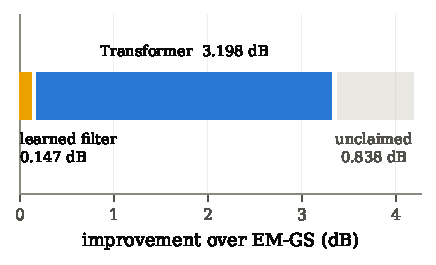
\includegraphics[width=0.94\columnwidth]{fig/fig1_attribution.pdf}
\caption{Where the unrolled estimator's gain over EM-GS comes from, at 80{,}000
training samples. The remainder is the gap to the genie-aided least-squares
reference, which is a reference and not a bound.}
\label{fig:attr}
\end{figure}

\subsection{Correcting the Loss}

The imbalance is a property of the loss, so we fix the loss. The remedy is
already known~\cite{wiesmayr2023bler}; this subsection reports what it is worth
in this setting. It is placed first only because the rest of the section is
easier to read once the loss is corrected.

The weighting works as intended. The realized per-bin gradient share spans a
factor of $1.9$ after balancing against $30.0$ before, and the share below
$5$~dB falls from $0.897$ to $0.427$ against an ideal of $0.5$. It slightly
over-corrects.

Against identically trained unbalanced networks, balancing gains $+1.902$,
$+2.242$ and $+2.369$~dB above $5$~dB on the three seeds, a mean of
$\mathbf{+2.171}$~dB. The standard deviation over seeds is $0.241$~dB, and the
seed interval is $[+1.572,+2.771]$~dB, which excludes zero.

We had predicted, in advance, a low-SNR \emph{cost} of $-0.10$ to $-0.40$~dB,
reasoning that the lowest bin's weight falls about eighteenfold. There was no
cost.

\subsection{Every Bin and Every Seed}

The obvious objection to a reweighting is that it simply moves accuracy from
one region to another: whatever the high-SNR bins gain, the down-weighted
low-SNR bins must have paid. Here they did not, and the check is exhaustive
rather than pooled.

Fig.~\ref{fig:allcells} plots every SNR bin for every seed. All eighteen
bin-by-seed point estimates favour the balanced loss, and seventeen of them
have a test-set interval that excludes zero. The single exception is seed~1's
$[-5,0)$~dB bin at $+0.044$~dB. The three-seed means rise from $+0.052$~dB in
$[-10,-5)$ to $+3.120$~dB in $[15,20)$.

The two lowest bins are the ones that matter for the objection, because the
weighting divides their contribution by about $18$ and $9$. They improve
anyway.

A reading of why, offered as a hypothesis and not as a result: under the
per-sample loss the low-SNR tail may dominate so strongly that the network is
underfitted \emph{everywhere}, in which case rebalancing stops wasting capacity
rather than moving it. We have not tested that, and the measurement should not
be read together with the explanation. Note also that these are eighteen
individual intervals, not a simultaneous statement about all of them at once,
and that a positive median in a bin does not guarantee a smaller expected
squared error there.

\begin{figure}[!t]
\centering
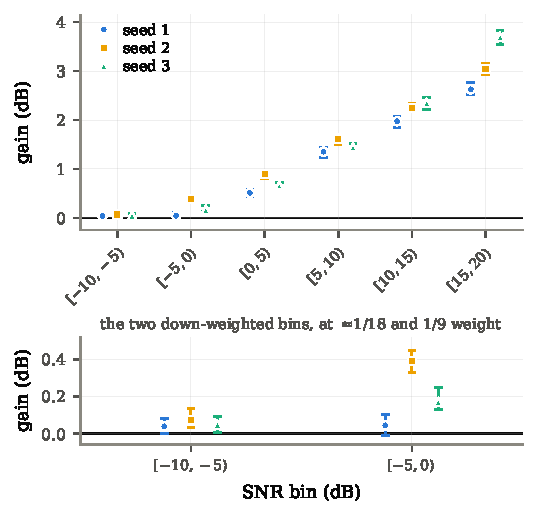
\includegraphics[width=0.94\columnwidth]{fig/fig5_allcells.pdf}
\caption{Every bin, every seed. The gain from balancing the loss, with test-set
intervals, for each of three training seeds. All eighteen are positive,
including the two lowest bins, whose weights the balancing divides by about
$18$ and $9$.}
\label{fig:allcells}
\end{figure}

\subsection{The Structural Gain Under Three Training Designs}
\label{sec:prior}

We now apply the control. Table~\ref{tab:designs} is the central measurement of
this paper. The structural step, the architecture, the data budget, the pilot
count and the test set are identical across its three rows. The only thing that
changes is how training distributed its effort.

\begin{table}[!t]
\caption{The structural gain $\Delta_H$ above $5$~dB under three training
designs, three seeds each. Positive means the structural step helps. Intervals
are over training seeds, not over the test set.}
\label{tab:designs}
\centering
\footnotesize
\setlength{\tabcolsep}{4pt}
\begin{tabular}{lccc}
\toprule
Training design & $\Delta_H$ (dB) & SD over seeds & $95\%$ seed interval \\
\midrule
Conventional loss & $\mathbf{+1.286}$ & $0.072$ & $[+1.107,+1.465]$ \\
Focused $[5,20]$ & $+0.020$ & $0.083$ & $[-0.187,+0.226]$ \\
Balanced loss & $-0.177$ & $0.150$ & $[-0.549,+0.196]$ \\
\midrule
\multicolumn{4}{l}{\emph{Paired change from conventional training}}\\
Focused $-$ conventional & $\mathbf{-1.267}$ & $0.124$ & $[-1.574,-0.959]$ \\
Balanced $-$ conventional & $\mathbf{-1.463}$ & $0.179$ & $[-1.908,-1.018]$ \\
\bottomrule
\end{tabular}
\end{table}

Read one row at a time, the three designs give a clearly positive value, a
value near zero, and a negative value.

Read as \emph{paired differences}, the result is much sharper. The three
designs use the same three seeds, so we can subtract seed by seed rather than
comparing three separate averages. Doing that, the change from conventional
training is $-1.267$~dB for focused retraining and $-1.463$~dB for the balanced
loss. Both intervals exclude zero, with $p=0.003$ and $p=0.005$ from a paired
$t$-test on two degrees of freedom.

\textbf{The change is what this experiment establishes. The endpoints are
not.} On three seeds, the focused and balanced values are each consistent with
zero, as their intervals in Table~\ref{tab:designs} show. We therefore do not
claim that the structural gain is absent under focused training, nor that it is
reliably negative under the balanced loss. What the paired comparison does
support, strongly, is that the measured gain moves by more than a decibel when
only the training design changes.

It is worth being clear about what this does and does not mean for the
structural step. A constraint can give a real improvement at a fixed training
budget, through easier optimization or through regularization, even if that
improvement disappears when the training is changed. That is still useful. The
distinction is between a benefit that depends on the training design and an
advantage that does not, and this experiment separates the two rather than
denying the first.

We also did not measure $\Delta_H$ under the log-domain loss of
Section~\ref{sec:logloss}, because that would need a structured network trained
with that loss, which we did not train. Three designs are reported here, not
four.

\subsection{A Single Number Hides a Sign Change}

Reported as one number, $\Delta_H$ is a weighted average of two opposite
effects. Table~\ref{tab:signs} shows the per-bin values.

\begin{table}[!t]
\caption{Per-bin structural gain $\Delta_H$, three-seed mean, under all three
training designs. A dash means the design never saw that bin. All eighteen
underlying cells of the conventional design --- three seeds by six bins --- have
a test-set interval excluding zero.}
\label{tab:signs}
\centering
\footnotesize
\begin{tabular}{lrrr}
\toprule
SNR bin (dB) & Conventional & Focused & Balanced \\
\midrule
$[-10,-5)$ & $-0.120$ & --- & $-0.233$ \\
$[-5,0)$ & $-0.400$ & --- & $-0.704$ \\
$[0,5)$ & $-0.293$ & --- & $-0.944$ \\
$[5,10)$ & $+0.457$ & $-0.173$ & $-0.692$ \\
$[10,15)$ & $+1.403$ & $+0.067$ & $-0.241$ \\
$[15,20)$ & $+2.290$ & $+0.259$ & $+0.567$ \\
\bottomrule
\end{tabular}
\end{table}

The structural step \emph{costs} accuracy at low SNR and \emph{buys} it at high
SNR. The sign changes exactly once.

Two things follow, and they behave differently.

\textbf{The ordering repeats; the crossing point does not.} On every arm we
have measured, every negative bin comes before every positive bin. On all three
conventional seeds the sequence is exactly $-,-,-,+,+,+$, and all eighteen
intervals exclude zero. But the bin at which the sign turns moves by up to two
positions between training designs. The ordering is the property that survives;
the crossing SNR is not, and neither is any single number that depends on where
it falls.

\textbf{The size falls under matched training, but the shape does not.}
Comparing the focused column against the conventional one, the two highest bins
shrink by factors of about $21$ and $9$, while the $[5,10)$ bin changes sign
rather than shrinking, from $+0.457$ to $-0.173$~dB. The balanced column is the
same story carried further: only the highest bin stays positive, and it is down
from $+2.290$ to $+0.567$~dB. In both corrected designs the top of the range
keeps a positive gain and the rest of the range does not.

\subsection{How the Average is Taken Decides the Sign}

Because the per-bin contributions have opposite signs, the number one reports
depends on the window the average is taken over. This includes which bins are
inside it and how the trials are combined within it.

There are two natural ways to combine trials. The \emph{paired median} takes
the improvement in each trial and reports the middle value, so every trial
counts equally. The \emph{ratio of sums} adds up the squared errors of both
methods and compares the totals, so a trial with a large error counts more.
Across three seeds of each design:

\begin{itemize}
\item conventional training, restricted to SNR~$\ge5$: $+1.209$, $+1.351$,
$+1.298$~dB by paired median; $+0.723$, $+0.856$, $+0.901$~dB by ratio of sums.
Positive under both.
\item conventional training, over the whole range: $+0.129$, $+0.225$,
$+0.196$~dB by median; $-0.214$, $-0.146$, $-0.141$~dB by ratio of sums. The
two \emph{disagree in sign}.
\item focused training, SNR~$\ge5$: $+0.078$, $+0.057$, $-0.076$~dB by median;
$-0.059$, $-0.077$, $-0.234$~dB by ratio of sums.
\end{itemize}

\textbf{The reason is measurable, and we measured it.} Sorting the trials by
the error of the unstructured network, the worst two deciles carry $51.2\%$ of
the total squared error and contribute $-0.134$~dB, while the remaining eight
deciles contribute almost nothing. That is not a separate effect of trial
difficulty: within a single SNR bin, the rank correlation between the baseline
error and $\Delta_H$ is $-0.009$, $-0.046$ and $+0.147$, against $-0.161$
overall and $+0.198$ against SNR itself. In other words, the sum of squared
errors is dominated by low-SNR trials, which is exactly where
Table~\ref{tab:signs} says the structural step costs accuracy.

\textbf{It is not the mechanism that produces the same symptom in the classical
estimator.} There, a selection rule declines to act on most trials, which pins
the median at zero. The unrolled network has no such rule: the step is applied
unconditionally, and it moves the estimate on every one of the $10$ layers of
every one of $2{,}000$ trials on every seed, with no trial anywhere near
inactive.

\subsection{A Simpler Loss, With No Resolved Difference}
\label{sec:logloss}

Per-bin reweighting needs bin edges, a measurement pass before training to
estimate the weights, and a choice of binning. Taking the per-sample error in
decibels before averaging needs none of these, because the logarithm divides
out the scale exactly, per sample. It is the obvious simplification, so we
tested it on three seeds.

Against the reweighted network it gains $+0.121$~dB above $5$~dB, with a
standard deviation over seeds of $0.131$ and a seed interval of
$[-0.204,+0.446]$~dB. That interval lies inside the $\pm0.50$~dB equivalence
margin we registered before these runs, so the pre-registered criterion for
equivalence is met. Stated without reference to that margin, \textbf{the
three-seed comparison simply does not resolve a difference.} Against the
conventional loss, both fixes gain about the same: $+2.290$~dB for the log
loss.

The log loss is not better balanced, either, and here our registered prediction
was wrong in the direction of the error. We had predicted that the log loss
would over-correct \emph{less} than per-bin reweighting. It over-corrects more:
its realized share of gradient below $5$~dB is $0.317$ to $0.329$ against an
ideal of $0.5$, where per-bin reweighting reaches $0.427$, and its span is $3.6$
against $1.9$. Dividing out the scale exactly does not equalize the gradient,
because the derivative of a logarithm is itself inversely proportional to the
error.

\textbf{This also limits our own diagnostic.} The same log-trained networks,
scored under the conventional loss, put $0.906$ to $0.911$ of the gradient
below $5$~dB with a span above $40$. These networks perform well and are not
undertrained in any way we can detect. A skewed gradient share therefore cannot
certify that training was inadequate, and the first step of the control in
Section~\ref{sec:protocol} should be read as a prompt to check, not as a test
that returns a verdict.

\subsection{Pilot Efficiency is not Pilot-Count Generalization}

A pilot-count curve for a trained estimator can mean two different things. It
can be one model trained at some $P_0$ and evaluated at each $P$, which
measures generalization. Or it can be a separate model trained at each $P$,
which measures efficiency. These are not close.

Trained at $P=10$, the estimator beats the $P=20$ model evaluated there by
$+2.231$~dB pooled, with every bin's interval excluding zero. At $P=35$ the
corresponding margin is $+0.635$~dB, so the model generalizes upward in pilot
count much better than downward.

At $5$~dB the matched-trained estimator reaches $-7.52$~dB at $P=10$, within
$0.47$~dB of the genie-aided reference, while the $P=20$ model evaluated there
is $2.60$~dB short of it. The $P=20$ model is also no better at $P=25$
($-11.13$~dB) than at $P=20$ ($-11.27$~dB). That difference is $0.14$~dB and we
report it without paired uncertainty, so it shows the absence of the expected
improvement rather than established harm from extra measurements.

This matters for how such curves are reported. The pilot sweep
of~\cite{xiao2026} does not state whether the networks were retrained per pilot
count. We report that as a fact about what the paper specifies, and as
motivation for stating the distinction, not as a criticism of that work, whose
convention is the ordinary one and which our own earlier curves shared.

\begin{figure}[!t]
\centering
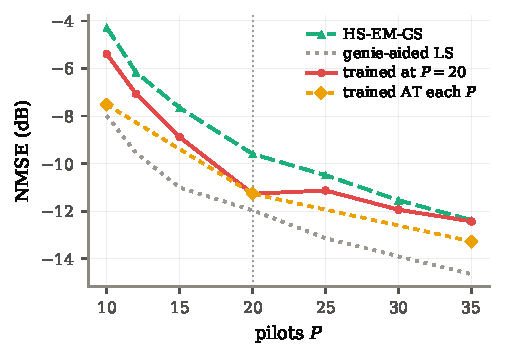
\includegraphics[width=0.94\columnwidth]{fig/fig4_pilots_three_way.pdf}
\caption{Pilot efficiency against pilot-count generalization at $5$~dB, on
identical realizations. The dashed diamonds are separate networks trained at
each $P$; the solid curve is one network trained at $P=20$.}
\label{fig:pilots}
\end{figure}

\section{Limitations and Conclusion}

A training loss averaged over a wide SNR range is dominated by its low-SNR
tail~\cite{wiesmayr2023bler}. In our setting $89.7\%$ of the measured gradient
falls below $5$~dB. The consequence we draw is about evidence rather than about
performance: a mechanism that improves high-SNR behaviour can appear to add
information it need not have supplied, so an uncontrolled comparison does not
establish that a structural constraint supplied it.

Applied to our own Hankel-structured estimator, the control moves a $+1.286$~dB
advantage by $-1.27$~dB under focused retraining and by $-1.46$~dB under a
corrected loss, measured as paired per-seed differences with intervals
excluding zero. Three designs, three seeds each, with nothing changed but how
training distributed its effort. The endpoints themselves are not separated
from zero on three seeds, and we do not claim them as absent or negative.

Two properties survive that a single number does not report: a per-bin sign
pattern that repeats across training designs and seeds while its crossing point
does not, and a dependence of the reported sign on how the average is taken.
Correcting the loss is an adaptation of a published remedy and is worth
$+2.171$~dB across three seeds here, improving all eighteen bin-by-seed point
estimates. A log-domain loss that needs no bin edges gives no resolved
difference from it.

\textbf{Limitations.} All results are simulation only, with no measured
hardware and no recorded channel data. They cover the geometric ULA model of
\eqref{eq:chan} at $N=32$, $K=3$, one data budget and the pilot counts tested.

Three seeds is few. The paired analysis makes three go further than three
separate estimates would, but it does not make three many, and every interval
over seeds in this paper rests on two degrees of freedom.

We have not shown that the networks trained with the conventional loss were
converged. Thirteen epochs with early stopping is a fixed budget, not a proof
of adequacy. If longer training on the conventional objective removed the
contrast, that would support an undertraining explanation; if it did not, the
result would be about the choice of objective instead. We have not run that
experiment, and the two readings are currently not separated.

The two interventions are also not fully independent. Both raise the relative
weight of the high-SNR region where the comparison is made, so their agreement
establishes that the measured gain depends on the training design. It does not
identify which of undertraining, objective alignment or sample allocation is
responsible.

Finally, the result is scoped to the structural step defined in
Section~\ref{sec:model}, applied unconditionally at every layer with a fixed
rank. A structural estimator that decides when to apply itself is a different
method and is not tested here.

\subsection*{Data and Pre-Registration Records}

Every prediction called pre-registered above exists as a dated record written
before the corresponding runs started. Each record fixes the threshold, the
falsifier and the rule that would decide the outcome, and each was scored held
or failed after the runs finished. The records, the scoring scripts and the
per-run result files accompany this manuscript. Two of the predictions in this
paper failed and are reported as failures in the text: the predicted low-SNR
cost of balancing, and the prediction that the log-domain loss would correct
the gradient share less than per-bin reweighting does.

\begin{thebibliography}{99}

\bibitem{gregor2010} K.~Gregor and Y.~LeCun, ``Learning fast approximations of
sparse coding,'' in \emph{Proc. Int. Conf. Mach. Learn. (ICML)}, 2010,
pp.~399--406.

\bibitem{monga2021} V.~Monga, Y.~Li, and Y.~C.~Eldar, ``Algorithm unrolling:
interpretable, efficient deep learning for signal and image processing,''
\emph{IEEE Signal Process. Mag.}, vol.~38, no.~2, pp.~18--44, 2021.

\bibitem{xiao2026} J.~Xiao, J.~Wang, M.~Zeng, H.~Xu, X.~Li, and
A.~Nallanathan, ``Channel estimation for Rydberg atomic quantum receivers:
unrolled phase retrieval from holographic snapshots,'' \emph{IEEE Signal
Process. Lett.}, vol.~33, pp.~1696--1700, 2026.

\bibitem{cui2025} M.~Cui, Q.~Zeng, and K.~Huang, ``Towards atomic MIMO
receivers,'' \emph{IEEE J. Sel. Areas Commun.}, vol.~43, no.~3, pp.~659--673,
2025.

\bibitem{wiesmayr2023bler} R.~Wiesmayr, G.~Marti, C.~Dick, H.~Song, and
C.~Studer, ``Bit error and block error rate training for ML-assisted
communication,'' 2022, arXiv:2210.14103, v3, Mar.~2023.

\bibitem{jameel2024ofdm} A.~S.~M.~M.~Jameel, A.~Malhotra, A.~El~Gamal, and
S.~Hamidi-Rad, ``Deep OFDM channel estimation: capturing frequency
recurrence,'' 2024, arXiv:2401.05436.

\bibitem{xu2025} B.~Xu, J.~Zhang, Z.~Chen, B.~Cheng, Z.~Liu, Y.-C.~Wu, and
B.~Ai, ``Channel estimation for Rydberg atomic receivers,'' \emph{IEEE Wireless
Commun. Lett.}, vol.~14, no.~9, pp.~2957--2961, 2025.

\bibitem{gerchberg1972} R.~W.~Gerchberg and W.~O.~Saxton, ``A practical
algorithm for the determination of phase from image and diffraction plane
pictures,'' \emph{Optik}, vol.~35, pp.~237--246, 1972.

\end{thebibliography}

\end{document}
